% %% %%%%%%%%%%%%%%%%%%%%%%%%%%%%%%%%%%%%%%%%%%%%%%%%%%%%%%%%%%
% step-1.tex
%
% Author:  Mauricio Matamoros
% License: MIT
%
% %% %%%%%%%%%%%%%%%%%%%%%%%%%%%%%%%%%%%%%%%%%%%%%%%%%%%%%%%%%%
%!TEX root = ../practica.tex
%!TEX root = ../references.bib

% CHKTEX-FILE 1
% CHKTEX-FILE 13
% CHKTEX-FILE 46

\subsection{Paso 1: Alambrado}%
\label{sec:step1}

El proceso de alambrado de esta práctica considera dos circuitos.
El primer circuito (véase \Cref{fig:circuit-ac}) opera con corrente alterna e integra un detector de cruce por cero y un convertidor AC-AC con base en un TRIAC.
Ambos subcircuitos cuentan con optoacopladores que servirán como interfaz para una conexión segura al circuito de DC.

El segundo circuito (véase \Cref{fig:circuit-dc}) está encargado de detectar el cruce por cero y enviar la señal de activación al TRIAC en el momento oportuno de acuerdo con la potencia requerida por el usuario (el brillo del foco) mediante una interfaz gráfica.

\medskip
\begin{importantbox}{\large \textsc{Advertencia}}
	\begin{center}
		Asegúrese de que todos los cables para el circuito AC están perfectamente aislados.

		Las puntas expuestas son un riesgo de electrocución y quemarán su arduino y su Pi con un sólo roce.

		\medskip{}

		\textbf{Utilice cinta aislante.}
	\end{center}
\end{importantbox}

Para este fin, se alambra la señal del subcircuito detector de cruce por cero a un pin digital del RP2040 controlado por la PIO que iniciará una cuenta regresiva y enviará la señal de activación al TRIAC una vez transcurrido el tiempo de activación, obteniéndose así la potencia deseada.
Asimismo, el RP2040 recibirá de la Raspberry Pi via \IIC{} la potencia solicitada por el usuario mediante una interfaz web.

Cabe mencionar que, al ser un circuito completamente digital, a la GPIO de la Raspberry Pi podría configurársele un pin en modo interrupción para recibir la señal del detector de cruce por cero y otro para el envío de la señal de activación del TRIAC.
Sin embargo, el paquete \texttt{RPi.GPIO} para el control de la GPIO con Python no soporta el uso de interrupciones de timer en hardware, por lo que no es posible garantizar que la señal de activación del TRIAC será enviada sin retrasos,
y mucho menos que el ciclo de trabajo será periódico y preciso.
Es por este motivo que se utiliza un RP2040 como auxiliar.

\subsubsection{Circuito de potencia en AC}%
Alambre primero el circuito de corriente alterna de la \Cref{fig:circuit-ac} tras verificar los valores de las resistencias de los optoacopladores.
Considere que si la resistencia de gatillo es muy grande (ej. 10M$\Omega$), el optoacoplador no recibirá suficente corriente y no encenderá lo suficiente como para disparar el fotosensor.
Por otro lado, si la resistencia es demasiado pequeña el optoacoplador se quemará irremediablemente.

\begin{figure}[H]
	\centering
	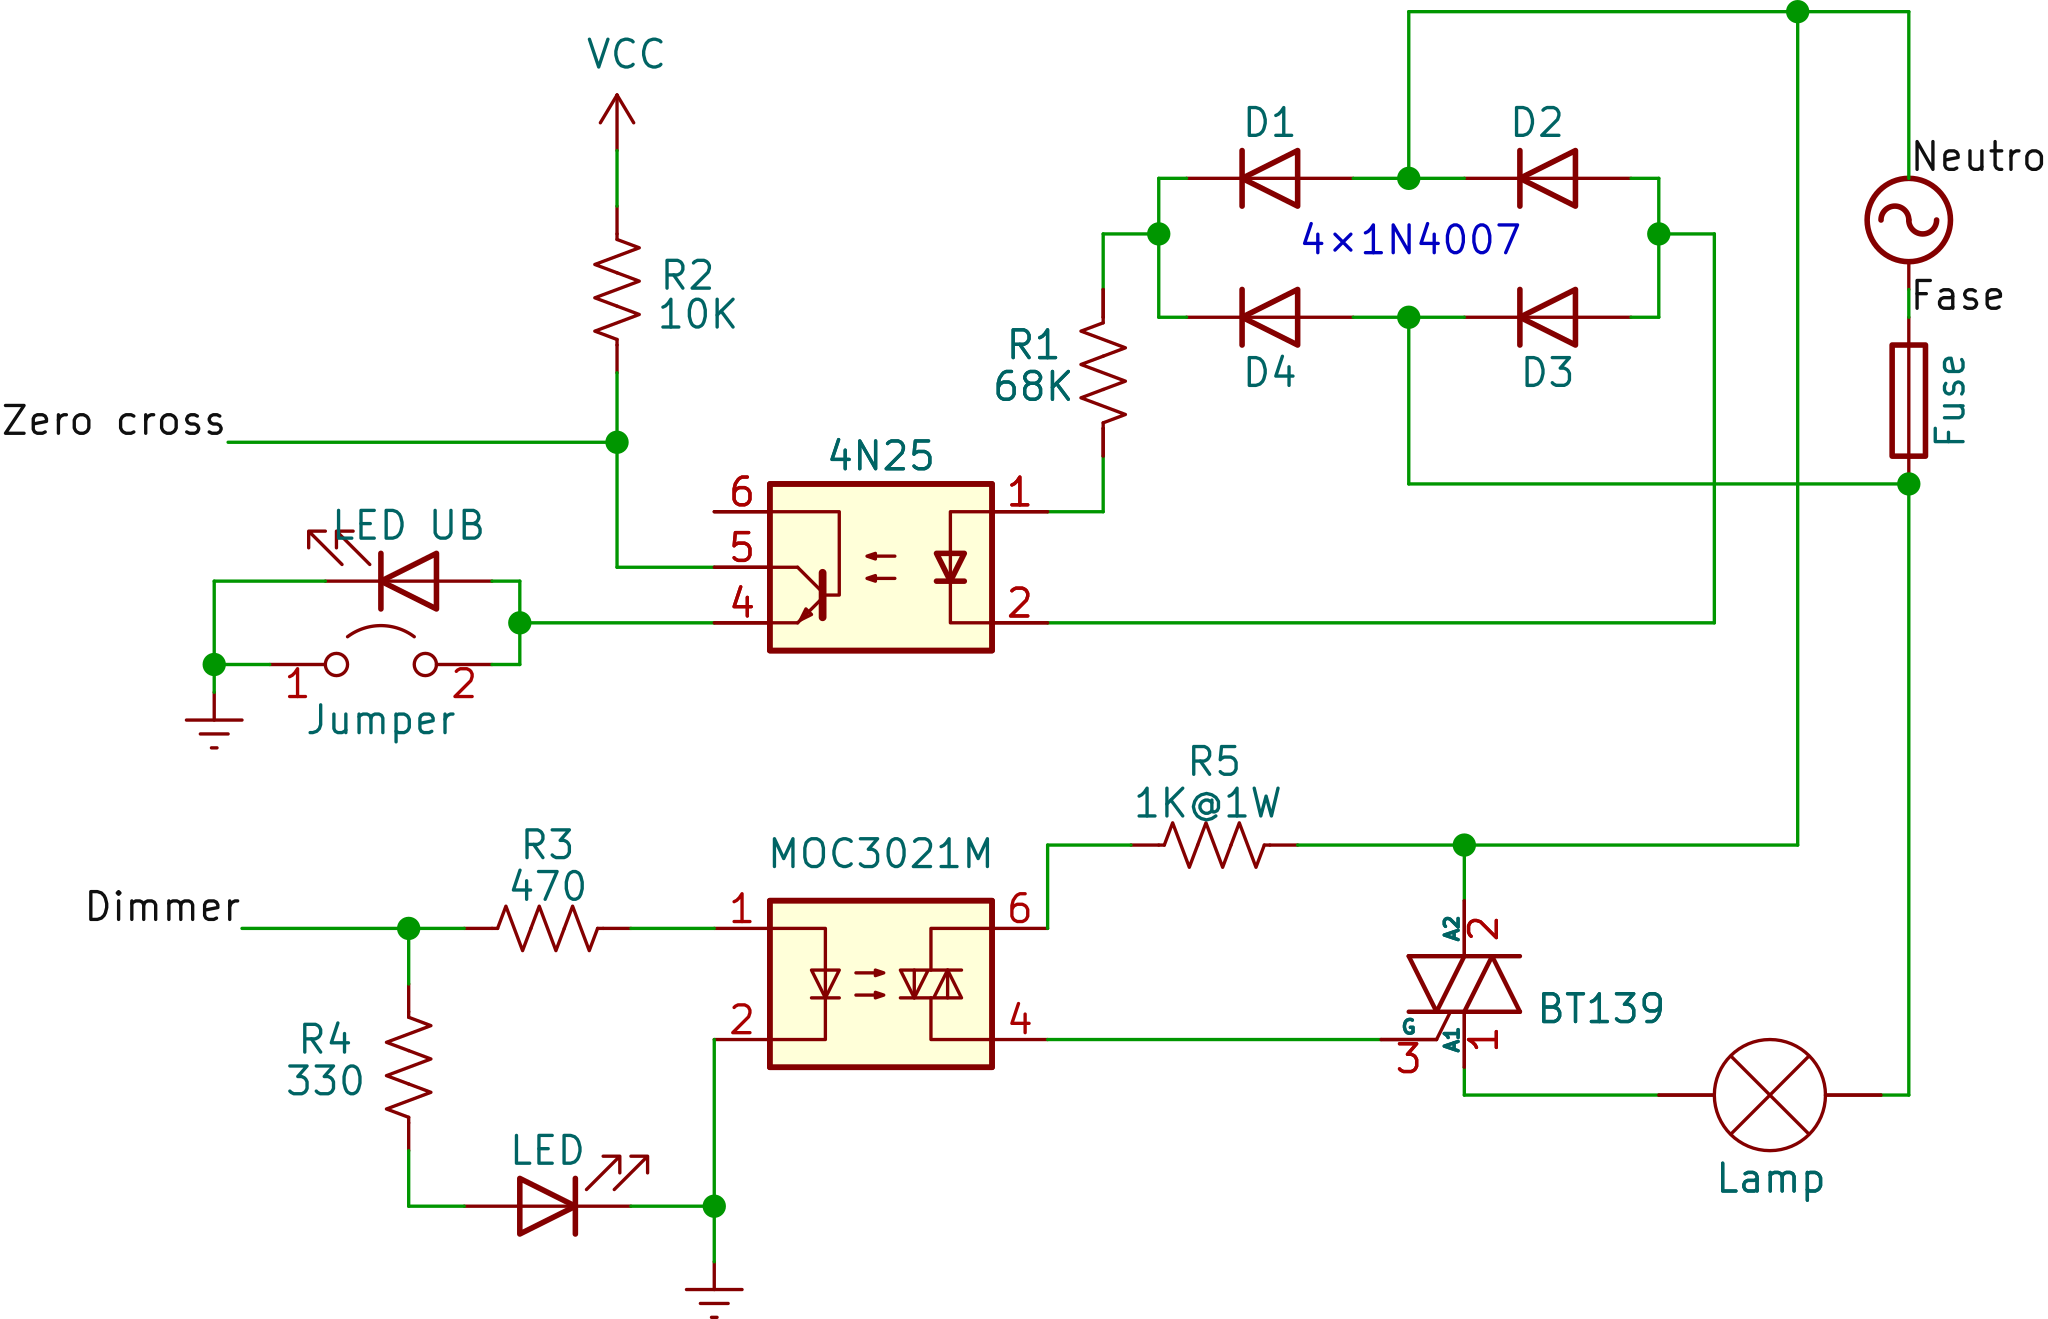
\includegraphics[width=0.5\columnwidth,height=7cm,keepaspectratio]{img/circuit-ac.png}
	\caption{Circuito de potencia en AC}%
	\label{fig:circuit-ac}
\end{figure}

Tras alambrar el circuito, es una buena idea probar el detector de cruce por cero con un osciloscopio, o al menos con un led ultrabrillante (LED UB), que deberá encender tenuemente.
De igual manera, conviene probar el encendido del foco inyectando 5V al MOC que acopla al TRIAC.

\medskip
\begin{importantbox}{\large Importante}
	\begin{center}
		Asegúrese de verificar con un multímetro que el circuito de AC está debidamente aislado y que no se tienen valores mayores a 5V en el segmento de DC.
		De otro modo podría quemar su RP2040 y su Raspberry Pi.
	\end{center}
\end{importantbox}

Continúe el alambrado del circuito.

\subsubsection{Circuito de control en DC}%
Alambre el circuito de corriente directa de la \Cref{fig:circuit-dc} tras verificar la tensión de las señales optoacopladas conectando el bus \IIC entre la Raspberry Pi y el RP2040 como ilustran la \Cref{tbl:pi-pico-i2c} y la \Cref{fig:circuit-dc}.
Hay tutoriales que sugieren utilizar un convertidor de niveles de voltaje cuando se conecta una Raspberry Pi a un RP2040 mediante \IIC.
Esto \textbf{NO} es necesario si la Raspberry Pi está configurada como dispositivo maestro o \emph{master} y el RP2040 como dispositivo esclavo o \emph{slave}.

\begin{figure}[H]
	\centering
	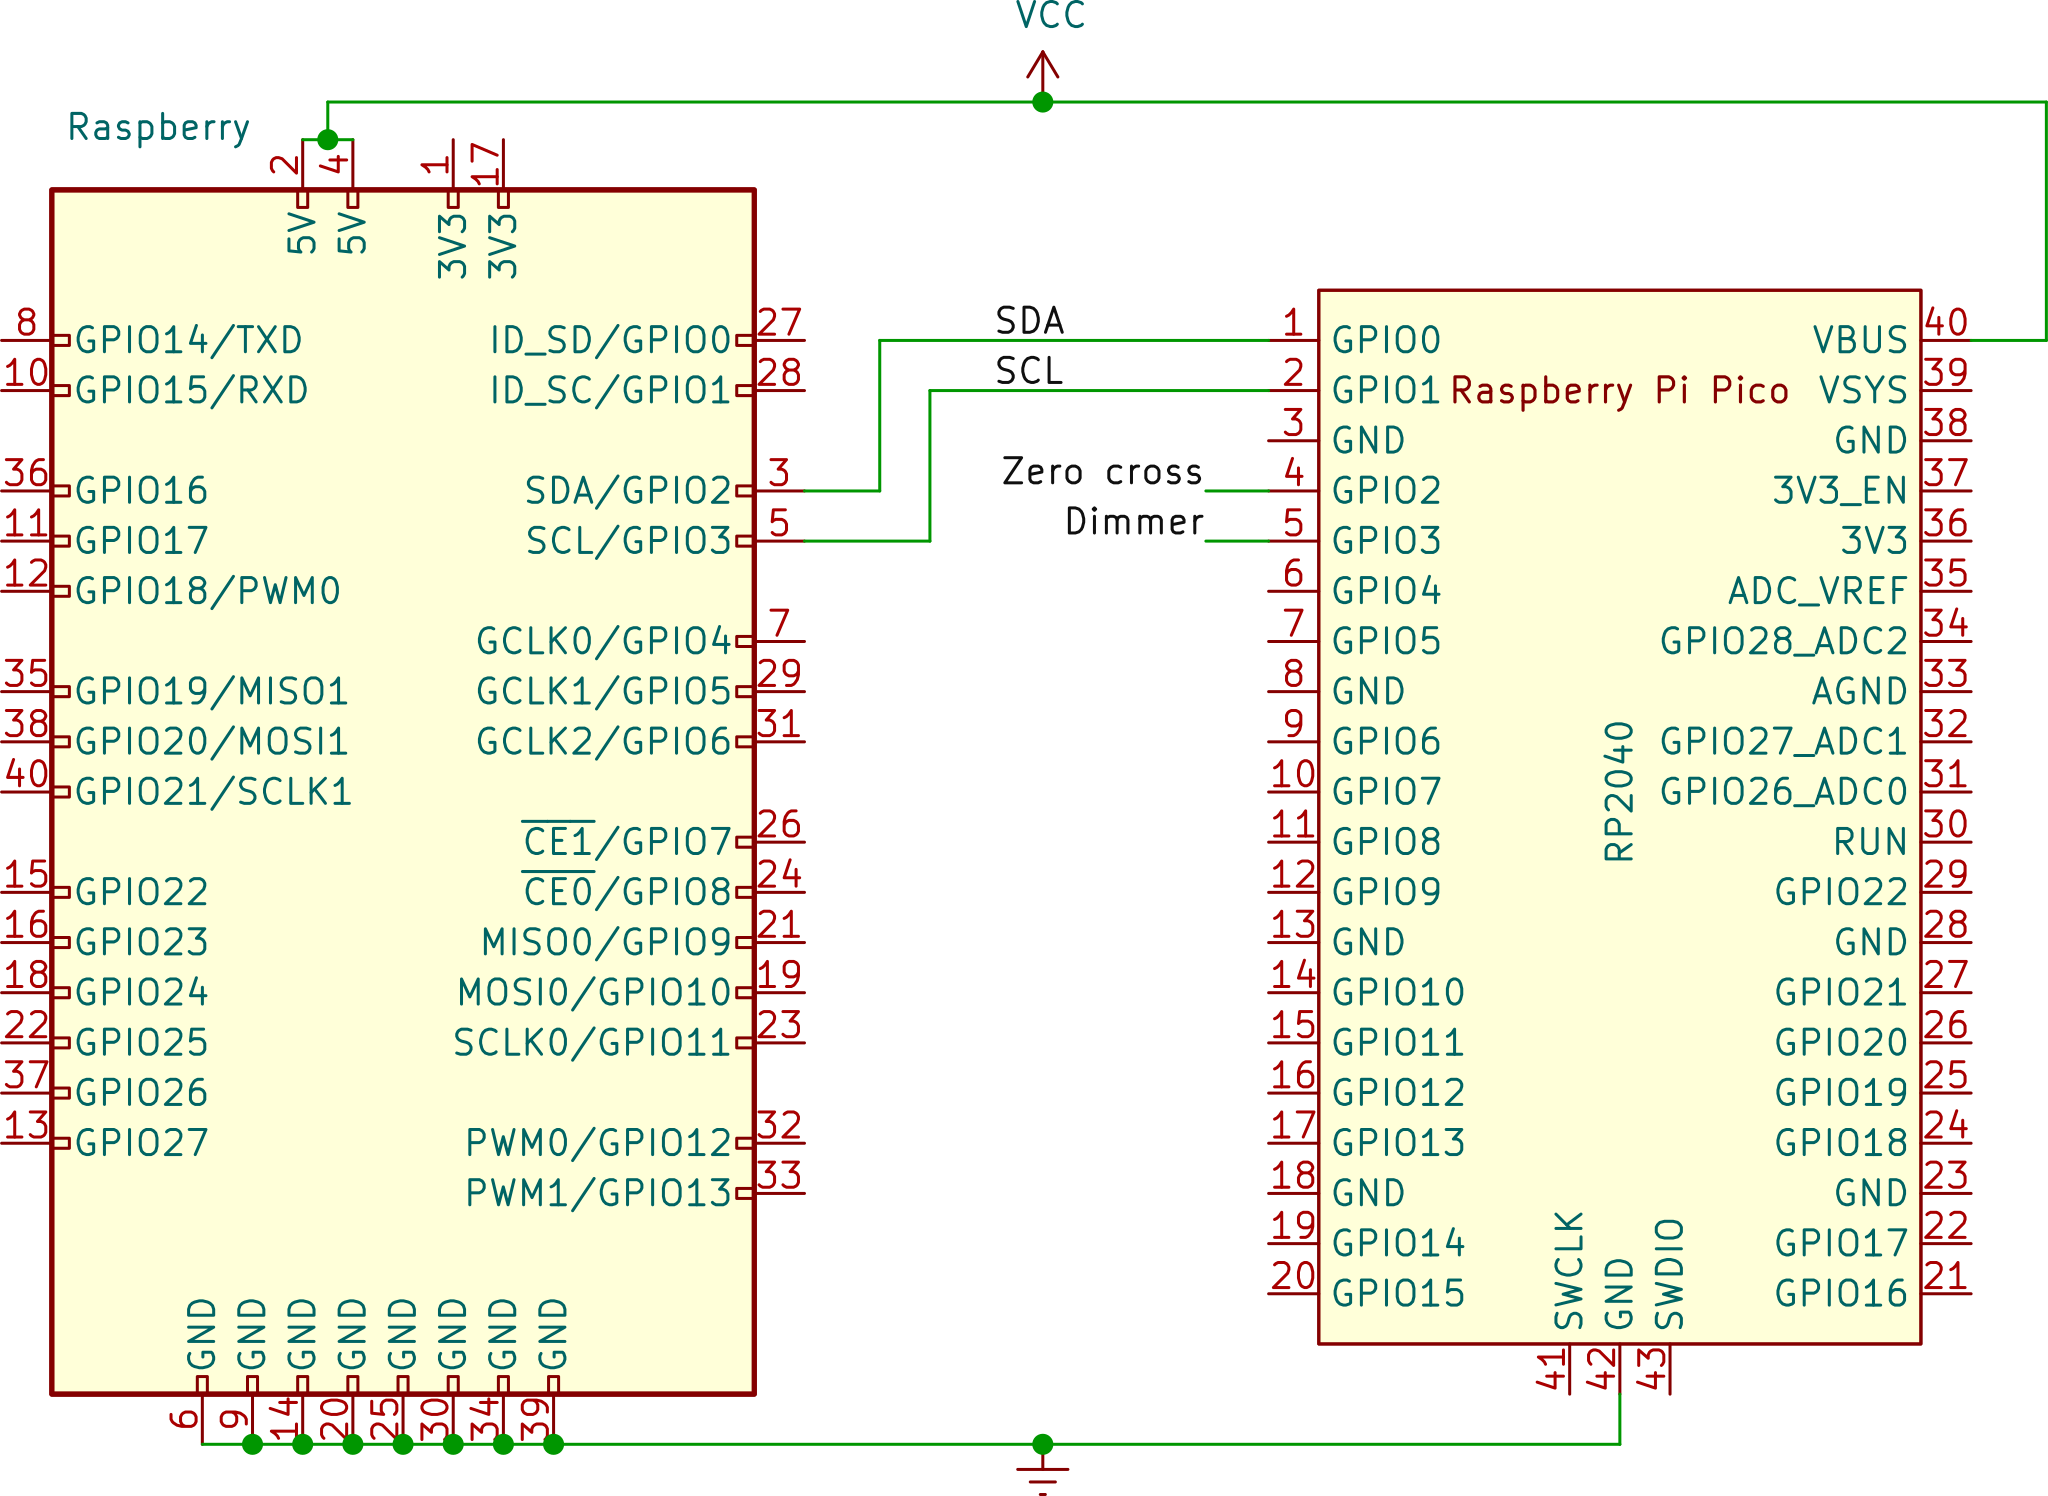
\includegraphics[width=0.5\columnwidth,height=7cm,keepaspectratio]{img/circuit-dc.png}
	\caption{Circuito de control en DC}%
	\label{fig:circuit-dc}
\end{figure}


\begin{table}
	\centering
	\caption{Conexiones \IIC entre Raspberry Pi y un RP2040}
	\label{tbl:pi-pico-i2c} % CHKTEX 24
	\begin{tabularx}{0.8\linewidth}{cc rcl cc }
	\toprule
	\multicolumn{2}{c}{   Pin   } & \multicolumn{3}{c}{\multirow{2}{*}{Conexión}}     & \multicolumn{2}{c}{  Pin   } \\
	\multicolumn{2}{c}{Raspberry} & \multicolumn{3}{c}{}                              & \multicolumn{2}{c}{ RP2040 } \\
	\midrule
	       3 & (GPIO2)            & Raspberry Pi SDA & \(\rightarrow{}\) & RP2040 SDA & GP0/GP20 & 1/26   \\
	       5 & (GPIO3)            & Raspberry Pi SCL & \(\rightarrow{}\) & RP2040 SCL & GP1/GP21 & 2/27   \\
	       6 & (\GND)             & Raspberry Pi GND & \(\rightarrow{}\) & RP2040 GND &   \GND   & 3/28   \\
	\bottomrule
	\end{tabularx}
\end{table}

Esto es posible debido a que el RP2040 no tiene resistencias de acoplamiento a positivo o \emph{pull-up} integradas, mientras que los pines \IIC de la Raspberry Pi están conectados internamente a la línea de 3.3V mediante resistencias de 1.8k\(\Omega{}\).
Por este motivo, tendrán que quitarse las resistencias de \emph{pull-up} a cualquier otro dispositivo esclavo que se conecte al bus \IIC de la Raspberry Pi.\footnote{Para más información sobre el papel de las resistencias de acoplamiento a positivo o \emph{pull-up} en un bus \IIC se puede consultar \url{http://dsscircuits.com/articles/effects-of-varying-i2c-pull-up-resistors} }

Un estudiante avispado habrá podido observar que en la \Cref{tbl:pi-pico-i2c} aparecen dos posibles pines para su uso como SDA, SCL y \GND{} en el RP2040.
De acuerdo con la hoja de especificaciones del fabricante, es posible utilizar cualquier pin entre el GP0 y el GP27 con excepción del GP22 para comunicaciones \IIC,
quedando repartidos los pines entre los periféricos \IIC{}0 e \IIC{}1 de forma alternada.
Es decir, \(2^{2n}\) y \(2^{2n}+1\) para el \IIC{}0
y
\(2^{2n+1}\) y \(2^{2n+1}+1\) para el \IIC{}1.


\medskip

A continuación pruebe el alambrado del circuito de DC con el programa de prueba del \Cref{sec:appendix1}.
El programa es muy simple, pues sólo configura interrupciones e imprime el conteo de estas.
Para activarlo inyecte repetidamente 5V con una resistenca de 1k$\Omega$ al pin de detección de cruce por cero.
Deberá observar en la pantalla la frecuencia de activación del pin en Hz.

Al terminar el alambrado debería tener completo el citcuito de la \Cref{fig:circuit-full}
\begin{figure}[H]
	\centering
	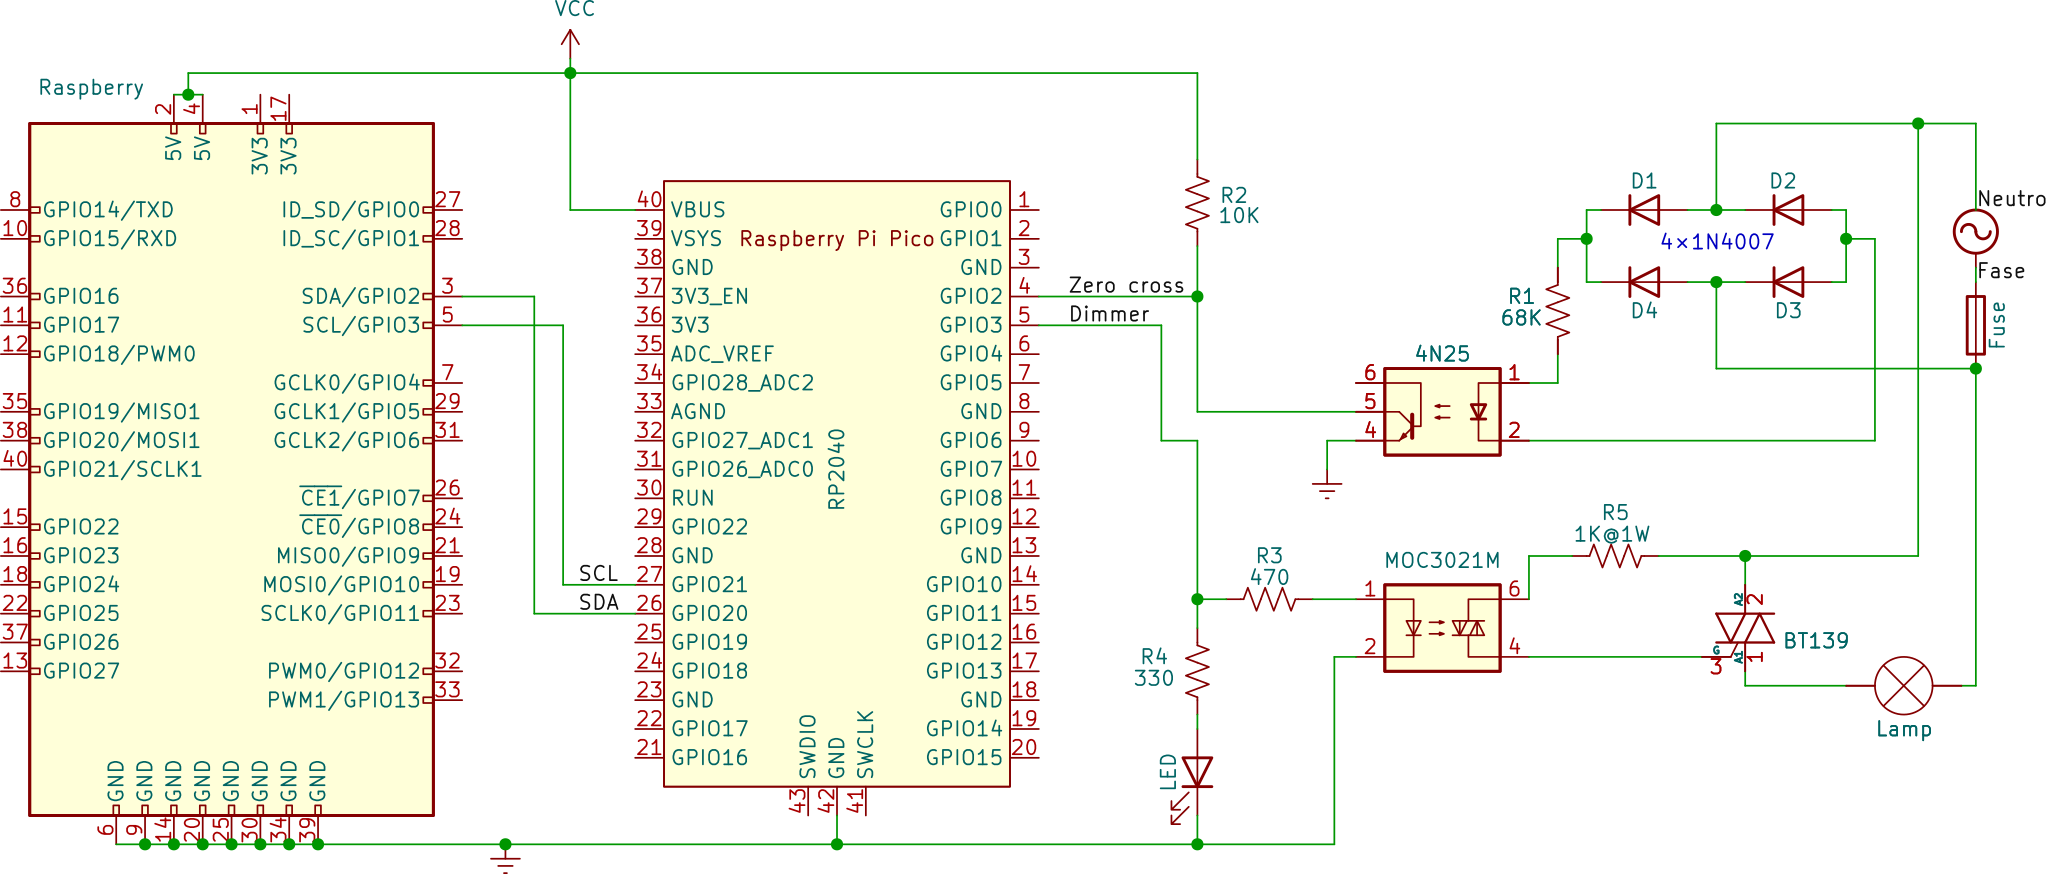
\includegraphics[width=0.75\columnwidth,height=9cm,keepaspectratio]{img/circuit-full.png}
	\caption{Diagrama de circuito alambrado completo}%
	\label{fig:circuit-full}
\end{figure}

Una vez alambrado, pruebe su circuito con el programa de prueba del \Cref{sec:appendix4}.
Dicho programa utiliza la máquina de estados de la PIO (\emph{\textbf{P}rogrammable \textbf{I}nput \textbf{O}utput}) del RP2040.
Este periférico permite programar los pines del RP2040 para descargar al procesador de las engorrosas tareas de transmisión y recepción de datos y que éste pueda enfocarse en realizar cómputo.

El uso de una PIO es necesario por un motivo fundamental:
al ser un lenguaje interpretado y orientado a objetos, Python hace un uso extensivo del \emph{heap} y de la pila cada vez que se llama a una función, reservando memoria de manera dinámica para todos los tipos, incluyendo enteros y flotantes.
La reserva de memoria dinámica es una operación de tipo \(O(n)\) respecto al tamaño de los objetos a reservar en la función, por lo que una simple llamada puede requerir de cientos o incluso miles de ciclos de reloj.
Además, como Python hace uso de la pila,\footnotemark{} lo que está prohibido al atender interrupciones, el intérprete encola las interrupciones para su ejecución concurrente a posteriori en lugar de atenderlas inmediatamente.
\footnotetext{%
	Toda declaración es una llamada implícita al constructor del objeto por lo que se hace uso de la pila con cada instrucción de Python.
	Además, cuando existe una relación de herencia, Python debe llamar al constructor de cada clase padre para instanciar al nuevo objeto, aumentando el número de \emph{push} a la pila.
}
Por otro lado, el uso de un PWM no es posible debido principalmente a la imposibilidad de sincronizar al periférico con el periodo de la onda de AC debido a la incertidumbre de esta última (los 50/60Hz no son necesariamente estables).
En contraste, el código de la PIO se traduce a un lenguaje tipo ensamblador que, una vez ensamblado, se inyecta al periférico para su ejecución autónoma.

Cada PIO cuenta con
	un PC o contador de programa,
	un registro de corrimiento de entrada o \emph{ISR (input Shift Register)},
	un registro de corrimiento de salida u \emph{OSR (Output Shift Register)},
	dos registros auxiliares \texttt{X} e \texttt{Y},
	y una lógica de control;
donde cada registro es de 32 bits.
Los registros de corrimiento son accessibles mediante colas síncronas de entrada y salida de 4 niveles, no así los registros auxiliares.

\clearpage

El autómata a cargar tiene siete estados como sigue:
\begin{enumerate}
	\item[\(q_0\).] \textbf{Inicialización y carga del retraso}\\
		Se apaga el TRIAC (pin en cero) y se espera a que haya datos en el \texttt{OSR}.\\
		Los datos del \texttt{OSR} (número de ciclos de espera) se copian al registro \texttt{X}.
		\par\noindent\begin{minipage}{\linewidth}
		\lstinputlisting[language=Python,
			title={\texttt{rp2040-test-acdc.py:24--26}},
			linerange={24-26}]{src/rp2040-test-acdc.py} %CHKTEX 8
		\end{minipage}

	\item[\(q_1\).] \textbf{Bucle. Espera por el cruce en cero}
		Se espera por un flanco de bajada en el pin de cruce por cero, indicando que el voltaje ha caído y la senoidal está en transición.
		\lstinputlisting[language=Python,
			title={\texttt{rp2040-test-acdc.py:29--33}},
			linerange={29-29,33-33}]{src/rp2040-test-acdc.py} %CHKTEX 8

	\item[\(q_2\).]  \textbf{Actualización del tiempo de espera}\\
		Se actualiza el valor de retardo copiando los datos de la cola de transmisión al registro \texttt{OSR}, si los hubiere (si no, OSR queda como está).\\
		Posteriormente los datos se transfieren a los registros auxiliares \texttt{X} e \texttt{Y}.
			\lstinputlisting[language=Python,
			title={\texttt{rp2040-test-acdc.py:36--38}},
			linerange={36-38}]{src/rp2040-test-acdc.py} %CHKTEX 8

	\item[\(q_3\).]  \textbf{Espera de transición}\\
		Se espera por un flanco de subida en el pin de cruce por cero, lo que indica que la transición ha terminado y el voltaje vuelve a subir.
		Posteriormente se realiza una espera de 4 ciclos de reloj (800\(\mu{}\)s) a fin de que haya suficiente voltaje para poder habilitar el TRIAC.
		\lstinputlisting[language=Python,style=py_without_comments,
			title={\texttt{rp2040-test-acdc.py:41--42}},
			linerange={41-42}]{src/rp2040-test-acdc.py} %CHKTEX 8

	\item[\(q_4\).]  \textbf{Espera activa (variación de potencia)}\\
		Se decrementa el registro \texttt{Y} hasta que llegue a cero.
		\lstinputlisting[language=Python,style=py_without_comments,
			title={\texttt{rp2040-test-acdc.py:48--49}},
			linerange={48-49}]{src/rp2040-test-acdc.py} %CHKTEX 8

	\item[\(q_5\).]  \textbf{Envío del pulso de encendido al TRIAC}\\
	Se envía un pulso de al menos 2\(\mu{}\)s al TRIAC para encenderlo.\\
	Como cada instrucción dura 200\(\mu{}\)s (cien veces más) una instrucción es más que suficiente.
		\lstinputlisting[language=Python,style=py_without_comments,
			title={\texttt{rp2040-test-acdc.py:52--53}},
			linerange={52-53}]{src/rp2040-test-acdc.py} %CHKTEX 8

\clearpage
	\item[\(q_6\).]  \textbf{Salto al estado \texttt{q1}}\\
	Se cierra el bucle regresando a la espera de cruce por cero.
		\lstinputlisting[language=Python,style=py_without_comments,
			title={\texttt{rp2040-test-acdc.py:56--56}},
			linerange={56-56}]{src/rp2040-test-acdc.py} %CHKTEX 8
\end{enumerate}

La máquina de estados se configura para operar a 5kHz (200\(\mu{}\)s por instrucción), lo que da aproximadamente 21 pasos por periodo, una variación de potencia aproximada del 5\% por cada paso asumiendo una progresión lineal.
